\documentclass[openany,12pt,UTF8]{ctexart}
\usepackage[a4paper,margin=2.5cm]{geometry}
\usepackage{amsmath}                                    % 排版数学公式

% 使equation计数器也依赖于section计数器
\numberwithin{equation}{section}

% 使table计数器也依赖于section计数器
\numberwithin{table}{section}

% 使figure计数器也依赖于section计数器
\numberwithin{figure}{section}

\usepackage{latexsym}
\usepackage{amsfonts}                                   %数学符号字体库宏包套件,它包含有:amsfonts、amssymb、eufrak 和 eucal 四个宏包。
\usepackage{amssymb}                                    % 定义AMS的数学符号命令
\usepackage{mathrsfs}                                   % 数学RSFS书写字体
\usepackage{bm}                                         % 数学黑体
\usepackage{graphicx}                                   % 支持插图,图形宏包graphics的扩展宏包
\usepackage{color,xcolor}                               % 支持彩色
\usepackage{amscd}
\usepackage[linesnumbered,ruled,vlined]{algorithm2e}
\usepackage{diagbox}
\usepackage{minted}
\usepackage{titlesec}                                   %设置章节格式
\usepackage{tcolorbox}

% 设置 paragraph 为只有一级编号(从1开始)
\renewcommand{\theparagraph}{\arabic{paragraph}} % 只显示一级编号
\makeatletter
\@addtoreset{paragraph}{section} % 每节开始时重置 paragraph 计数器
\makeatother

%%文本框设置
\newcommand{\tbox}[1]{
  \begin{center}
    \begin{tcolorbox}[colback=gray!10,%gray background
        colframe=black,% black frame colour
        width=14cm,% Use 8cm total width,
        arc=1mm, auto outer arc,
        boxrule=0.5pt,
      ]
      {#1}
    \end{tcolorbox}
  \end{center}
}

% 设置 paragraph 为 block 风格,自动换行
\titleformat{\paragraph}[block]
  {\normalfont\normalsize\bfseries}{\theparagraph.}{0.5em}{}

% 设置标题后换行(after-sep 设为 \newline)
\titlespacing*{\paragraph}{0pt}{3.25ex plus 1ex minus .2ex}{0pt}
  
\usepackage{enumerate}                                 	%更改enumerate环境格式
\usepackage{hyperref}

%改变超链接颜色
\hypersetup{
    colorlinks=true,
    linkcolor=blue,
    filecolor=blue,      
    urlcolor=blue,
    citecolor=cyan,
}

\usepackage{subcaption}
\usepackage{minipage-marginpar}
\usepackage{float}%提供float浮动环境
\usepackage{booktabs}%提供命令\toprule、\midrule、\bottomrule
\usepackage{listings}
\usepackage{xcolor}
\usepackage{tabularx}
\usepackage{multirow}
\usepackage[perpage]{footmisc}

% 自定义命令,用于角标引用文献和交叉引用
\newcommand{\scite}[1]{\textsuperscript{\cite{#1}}}
\newcommand{\sref}[1]{\textsuperscript{\ref{#1}}}
\newcommand{\bs}[1]{\boldsymbol{#1}}
\newcommand{\romannumber}[1]{\uppercase\expandafter{\romannumeral#1}}
\newcommand{\alert}[1]{\textcolor{red}{#1}}

% 设置标题层级和目录层级
\setcounter{tocdepth}{3}
\setcounter{secnumdepth}{4}
\usepackage{rotating}
\title{Simulation Practice Report for Statistics of Flight Experiment}
\author{Ouyang Jiahong}
\date{\today}
\begin{document}
\maketitle
\newpage
\tableofcontents
\newpage

\section{Introduction of the simulation task}
\subsection{背景}
\subsubsection{陀螺仪的测量模型}
\begin{equation}
    \label{equation:陀螺仪的测量模型}
    \omega_{G} = \underbrace{E_{\omega 0}}_{\text{Bias}} + \underbrace{E_{\omega 1}}_{\text{Factor}} \cdot (\omega + \text{Vel}_{ver}) + \varepsilon_{G}
\end{equation}

\subsubsection{输入数据}
\paragraph{角速度输入}\
\begin{equation}
    \omega = [60\ 40\ 50\ 80\ 33\ 24\ 17]^{\text{T}} \ (\circ/\text{s})
\end{equation}

\paragraph{测量噪声}\
\begin{equation}
    \varepsilon_{G} \sim N(0,\ 1 \times 10^{-8})
\end{equation}
即均值为0、方差为 $1 \times 10^{-8}$ 的高斯白噪声

\subsubsection{纬度与垂直方向角速度}
\paragraph{地理纬度(PhiN)}\
\begin{equation}
    \text{PhiN} = 28.209167\ ^\circ
\end{equation}
\paragraph{垂直方向角速度(考虑地球自转)}\
\begin{equation}
    \text{Vel}_{ver} = 7.292 \times 10^{-5} \times \text{r2d} \times \sin(\text{PhiN} \times \text{d2r})
\end{equation}
其中:
\begin{itemize}
    \item \texttt{r2d} 表示将弧度转换为角度(即 $180/\pi$)
    \item \texttt{d2r} 表示将角度转换为弧度(即 $\pi/180$)
\end{itemize}

\paragraph{采样步长}\

0.01秒

\subsection{任务}
\begin{enumerate}
    \item 请使用批量最小二乘法(Batch LS)和递推最小二乘法(RLS)来估计陀螺仪的偏差(bias)和标度因子(scale factor),并比较这两种估计方法的结果。
    \item 当使用批量最小二乘法(Batch LS)时,请估计测量噪声的方差。
    \item 当使用递推最小二乘法(RLS)时,请通过仿真回答以下问题:
          \begin{itemize}
              \item 当初始参数设置为批量最小二乘(BLS)解时,与初始参数随机设定时,估计误差曲线会如何变化?
              \item 参数估计误差曲线受初始条件的影响是怎样的?
          \end{itemize}
\end{enumerate}

\subsection{所提供的数据格式说明}
\subsubsection{GyroMeasData\_X.mat}
在\texttt{GyroMeasData\_X.mat}中,存储了500×7的double数据,每一组数据1×7代表了一组\(\omega\)观测数据。X代表了实验的组数,从0-100。我们要利用X组实验中的500次观测数据进行Bias和Factor的估计,估计式如\autoref{equation:陀螺仪的测量模型}所示。
\subsubsection{GyroBias.mat}
在\texttt{GyroBias.mat}中,存储了1×100的double数据,每一组数据代表了一个实验的Bias真值。例如GyroBias[1]代表了X=1时的Bias真值,也就是对应GyroMeasData\_1.mat的实验的真值。
在利用\texttt{GyroMeasData\_X.mat}的数据求解处\texttt{estimate\_{bias}}之后,要与真值进行对比。
\subsubsection{GyroFactor.mat}
在\texttt{GyroFactor.mat}中,存储了1×100的double数据,每一组数据代表了一个实验的Factor真值。例如GyroFactor[1]代表了X=1时的Factor真值,也就是对应GyroMeasData\_1.mat的实验的真值。
在利用\texttt{GyroMeasData\_X.mat}的数据求解处\texttt{estimate\_{factor}}之后,要与真值进行对比。


\section{Introduction of the algorithm investigated}

\section{Results and Analysis}

\subsection{Results of simulations}
\subsubsection{Residuals of Bias Estimation}
\autoref{figure:Residuals of Bias Estimation}是一张“偏差估计残差”(Residuals of Bias Estimation)的图表。横坐标为“实验编号”(Experiment Number),范围是0 - 50;纵坐标为“估计值 - 真实值”(Estimate - True),数量级为10⁻⁶ ,范围大致在 -4到8之间。图中有三种数据系列:
“BLS残差”(BLS Residuals),以蓝色圆点表示;
“RLS(随机初始)残差”(RLS (random initial) Residuals),用红色实线表示;
“RLS(BLS初始)残差”(RLS (BLS initial) Residuals),由绿色虚线呈现。

图中0值处有一条黑色虚线作为参考线,展示了不同方法的残差在各实验编号下的波动情况。 可以看到不同方法的残差在各实验编号下的波动情况都非常小,在1e-6以内。
\begin{figure}[h]\centering
    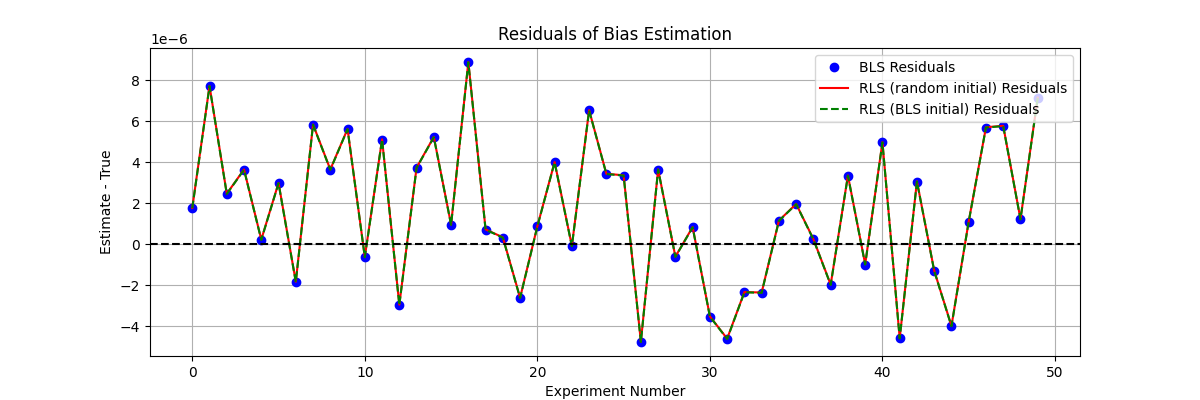
\includegraphics[width=\columnwidth]{figures/Residuals of Bias Estimation.png}
    \caption{Residuals of Bias Estimation}
    \label{figure:Residuals of Bias Estimation}
\end{figure}

\subsubsection{Residuals of Factor Estimation}
\autoref{figure:Residuals of Factor Estimation}一张“因子估计残差”(Residuals of Factor Estimation)的折线图和散点图。横坐标是“实验编号”(Experiment Number),范围从0到50;纵坐标是“估计值 - 真实值”(Estimate - True),范围约从 -2.0×10⁻⁷到1.0×10⁻⁷。图中有三种数据系列:
“BLS残差”(BLS Residuals),用蓝色圆点表示;
“RLS(随机初始)残差”(RLS (random initial) Residuals),用红色实线表示;
“RLS(BLS初始)残差”(RLS (BLS initial) Residuals),用绿色虚线表示。

可以看到不同方法的残差在各实验编号下的波动情况都非常小,在1e-7以内,0值处有一条黑色虚线作为参考线。 
\begin{figure}[h]\centering
    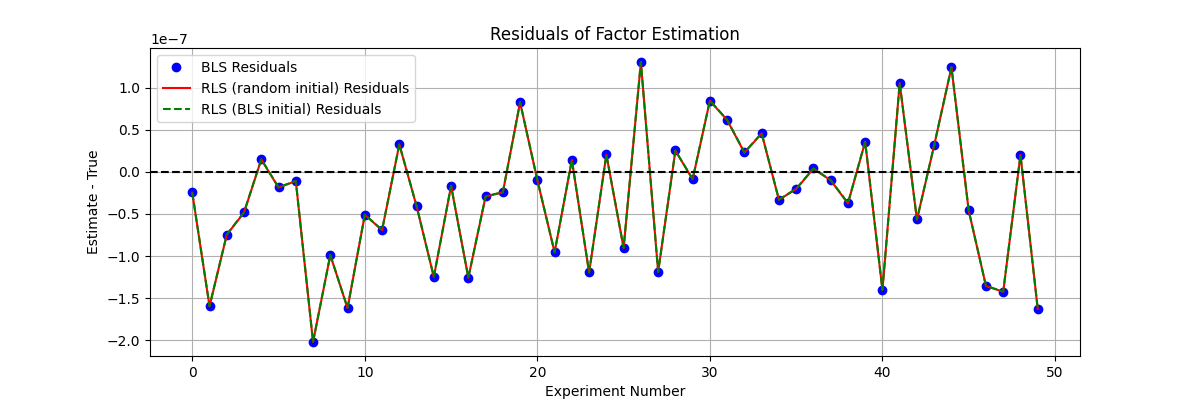
\includegraphics[width=\columnwidth]{figures/Residuals of Factor Estimation.png}
    \caption{Residuals of Factor Estimation}
    \label{figure:Residuals of Factor Estimation}
\end{figure}

\subsubsection{Bias and Factor Estimation of Exp 1}
\autoref{figure:Bias and Factor Estimation of Exp 1}包含两个子图,分别展示偏差估计收敛和因子估计收敛情况,均为实验1(Exp 1)的结果。可以看到,通过引入BLS的结果作为RLS的初值,可以稍微加快结果收敛的速度,但是在这个实验中显示的不明显。

左侧子图标题为“Bias Estimation Convergence - Exp 1”(偏差估计收敛 - 实验1)。横坐标是“Iteration Step”(迭代步骤),范围从0到8;纵坐标是“Bias Estimate”(偏差估计),范围从0到0.008。图中有三条线:
红色实线代表“RLS Random Init”(RLS随机初始化);
蓝色实线代表“RLS BLS Init”(RLS以BLS初始化);
黑色虚线代表“True Bias”(真实偏差)。

右侧子图标题为“Factor Estimation Convergence - Exp 1”(因子估计收敛 - 实验1)。横坐标同样是“Iteration Step”(迭代步骤),范围从0到8;纵坐标是“Factor Estimate”(因子估计),范围从 -0.00014到0。图中也有三条线:
红色实线代表“RLS Random Init”(RLS随机初始化);
蓝色实线代表“RLS BLS Init”(RLS以BLS初始化);
黑色虚线代表“True Factor”(真实因子)。 
\begin{figure}[h]\centering
    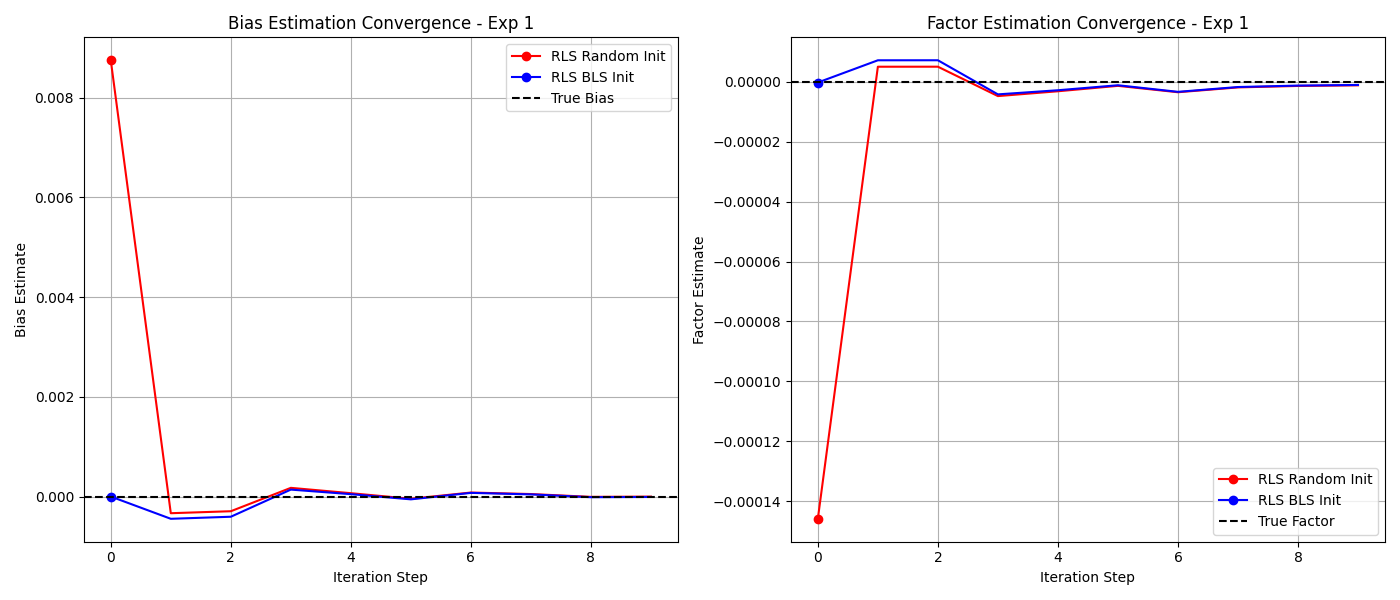
\includegraphics[width=\columnwidth]{figures/Bias and Factor Estimation of Exp 1.png}
    \caption{Bias and Factor Estimation of Exp 1}
    \label{figure:Bias and Factor Estimation of Exp 1}
\end{figure}

\subsubsection{Bias and Factor Estimation of All Exp}
\autoref{figure:Bias and Factor Estimation of All Exp}包含两个子图,分别展示所有实验的偏差估计收敛和因子估计收敛情况。可以看出,所有组实验数据的结果类似。

左侧子图标题为“Bias Estimation Convergence (All Experiments)”(所有实验的偏差估计收敛)。横坐标是“Iteration Step”(迭代步骤),范围从0到8;纵坐标是“Bias Estimate Error”(偏差估计误差),范围从0到0.008。图中有三种线条:
 红色线条代表“RLS Random Init”(RLS随机初始化);
 蓝色线条代表“RLS BLS Init”(RLS以BLS初始化);
 黑色虚线代表“True Bias”(真实偏差)。
有多条同色线条交织,显示多次实验的结果。

右侧子图
标题为“Factor Estimation Convergence (All Experiments)”(所有实验的因子估计收敛)。横坐标是“Iteration Step”(迭代步骤),范围从0到8;纵坐标是“Factor Estimate Error”(因子估计误差),范围从 -0.00015到0.000025。图中同样有三种线条:
红色线条代表“RLS Random Init”(RLS随机初始化);
 蓝色线条代表“RLS BLS Init”(RLS以BLS初始化);
 黑色虚线代表“True Factor”(真实因子)。
有多条同色线条交织,展示多次实验的结果。 
\begin{figure}[h]\centering
    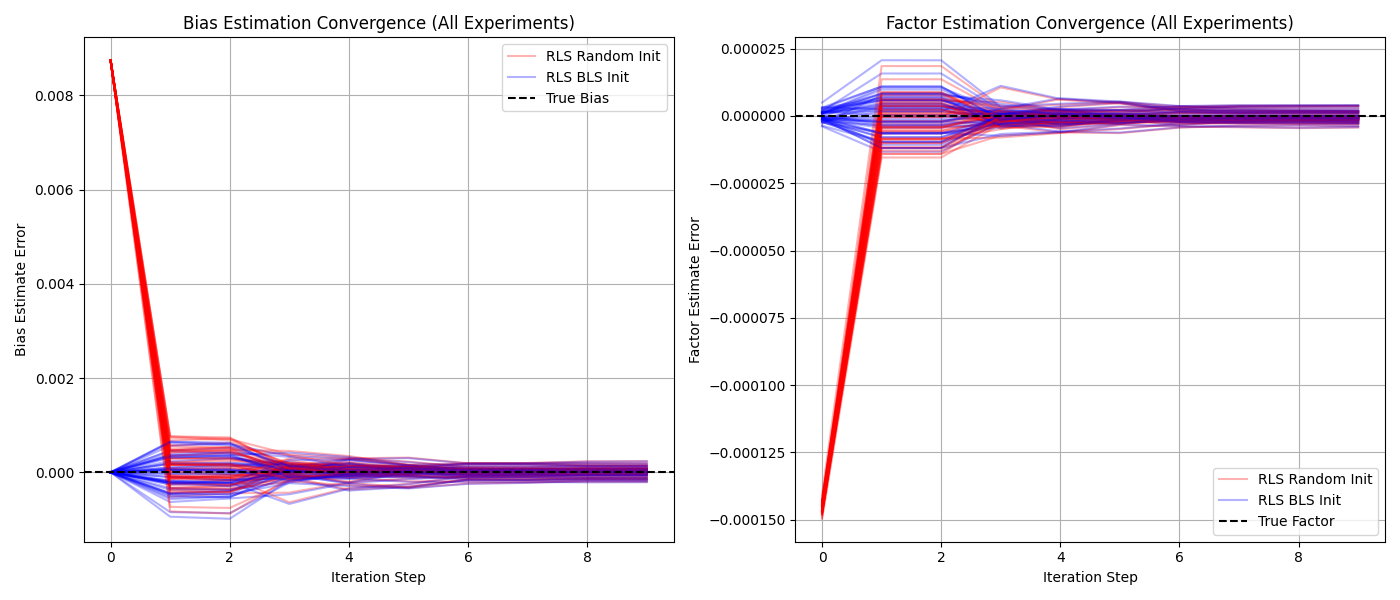
\includegraphics[width=\columnwidth]{figures/Bias and Factor Estimation of All Exp.png}
    \caption{Bias and Factor Estimation of All Exp}
    \label{figure:Bias and Factor Estimation of All Exp}
\end{figure}

\subsection{Analysis}

\section{Appendix}
Paste your code here.

\end{document}